As animações de diferentes tipos de ambientes físicos foram nossos primeiros resultados obtidos. Após desenhar alguns cenários simples que ilustravam tópicos da disciplina de física, como descrito na seção \ref{atividades}, partimos para implementação. Nosso principal objetivo nesta etapa era compreender melhor o funcionamento do Chipmunk: seus conceitos, seus recursos e suas limitações. \\

Além disso, como tínhamos em mente implementar um criador de cenários, a medida que implementávamos estas demonstrações extraíamos todo código relevante para classes auxiliares que pudessem ser reutilizadas posteriormente. Atualmente, a classe {\tt physics.rb} contém grande parte deste código extraído. \\

\begin{lstlisting}[language=Ruby, caption=Trecho de código do physics.rb]
# @param [Hash] options : mapa com as opcoes de 
#           configuracao do objeto fisico.
def setup_trait(options = {})
  self.color =  options[:color] || Gosu::Color::WHITE
  self.zorder = options[:zorder] || 100
  self.factor = options[:factor] || options[:scale] 
    || $window.factor || 1.0
  @visible = true   unless options[:visible] == false

  if options[:static]
    @body = CP::StaticBody.new
  else
    @body = CP::Body.new(options[:mass], 
        options[:moment_inertia])
    @body.v = options[:v] if options[:v]  
    @body.w = options[:rotational_velocity] || 0
    @body.add_to_space($space)
  end
  (...)
end
\end{lstlisting}

\subsection{Descrição}

\begin{figure}[H]
	\centering
	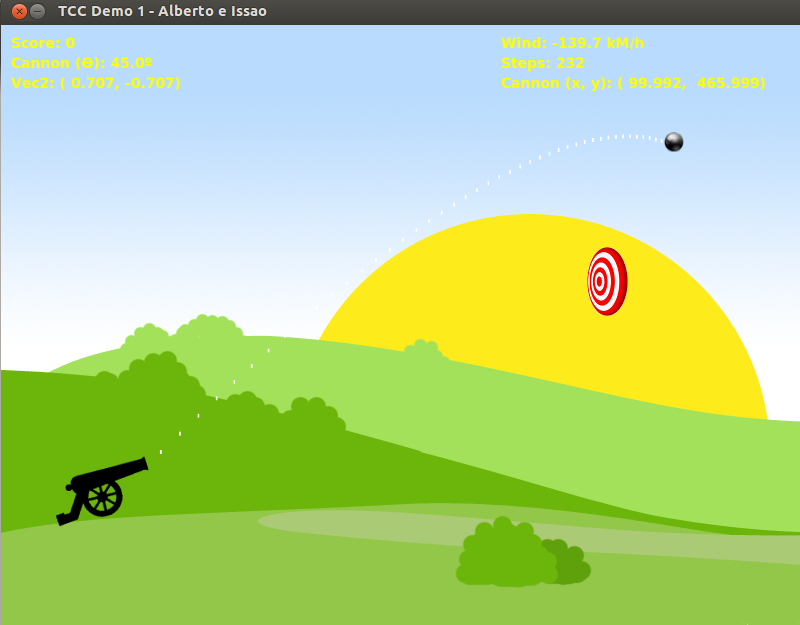
\includegraphics[scale=0.4]{images/cannonball.png}
	\caption{Cannonball}
	\hspace{0.5cm}
\end{figure}

\textit{Cannonball} foi nosso primeiro cenário físico. Baseado em jogos comuns de tiro ao alvo, como arco-e-flecha e catapultas, o objetivo é acertar uma bola de canhão em um alvo de posição escolhida aleatoriamente. O usuário pode modificar a angulação do canhão e atirar a bola pressionando a tecla de espaço. Há um vento de intensidade também calculada de forma aleatória, na direção horizontal e sentido contrário ao do trajeto da bola ao alvo. As informações relevantes ao usuário - ângulo do canhão, intensidade do vento, pontuação, entre outros - são exibidas no topo da janela. \\

Nossa intenção com este cenário era ilustrar o comportamento de lançamentos oblíquos e resistência do ar. \\

Posteriormente, utilizamos o código de \textit{Cannonball} na integração com exercício-programa \textit{Angry-Bixos}, descrita na seção \ref{ep}. \\

\newpage

\begin{figure}[H]
\centering
	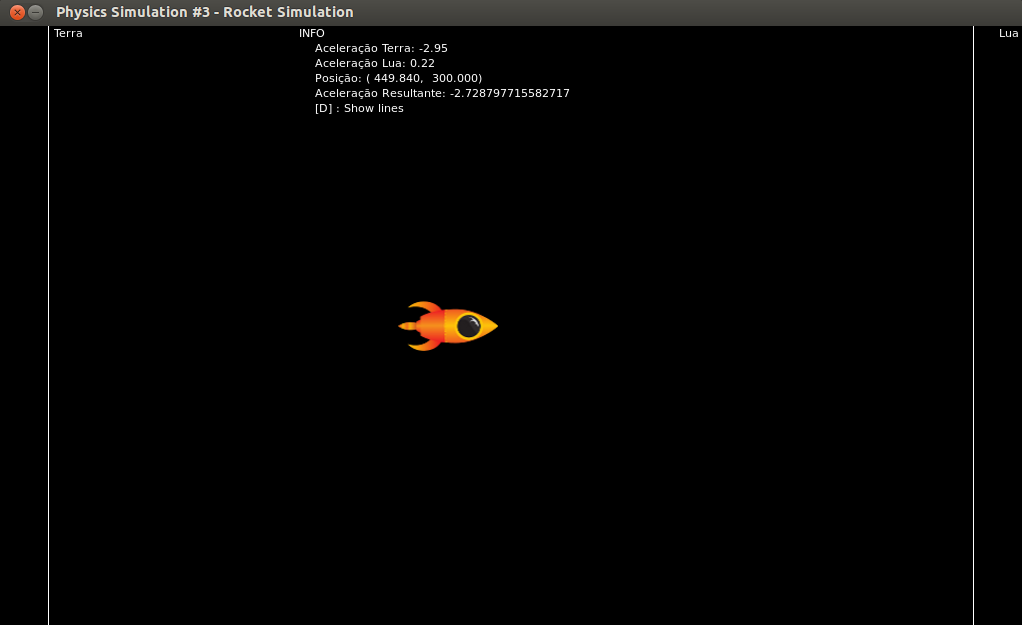
\includegraphics[scale=0.3]{images/rocket-simulation.png}
\end{figure}

\begin{figure}[H]
\centering
	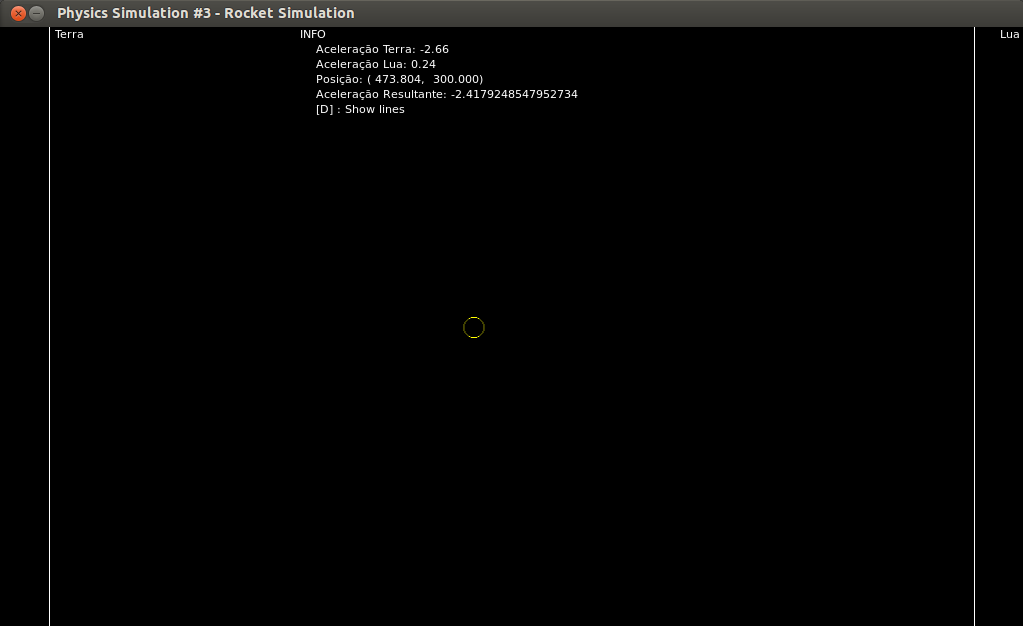
\includegraphics[scale=0.3]{images/rocket-simulationE.png}
	\caption{Rocket Simulation}
\end{figure}

A ação conjunta das gravidades da Terra e da Lua sobre um objeto é simulada em \textit{Rocket Simulation}. Controlando um foguete, o usuário pode movimentar-se com as setas do teclado entre os dois corpos, representados por retas nas extremidades esquerda e direita da tela. Por ter uma massa bem maior, a atração exercida pela Terra é maior em boa parte da tela, exceto em regiões bem próximas à Lua. \\

Por motivos de simulação, não reproduzimos os valores reais de massa de ambos os corpos, pois a região em que a Lua teria maior efeito sobre a nave seria ínfima e não proporcionaria ao usuário a experiência que gostaríamos. \\

\begin{figure}[H]
\centering
	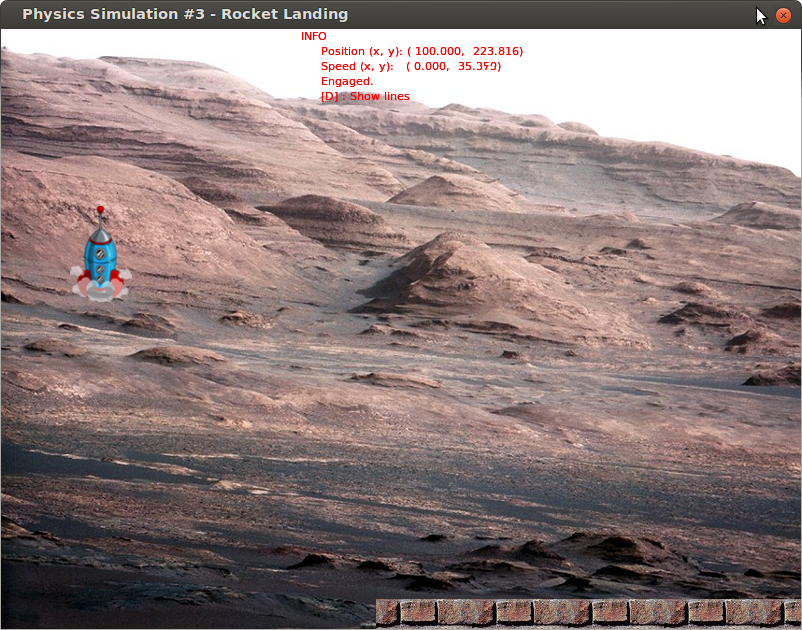
\includegraphics[scale=0.4]{images/lunarLanding.png}
\end{figure}
\begin{figure}[H]
\centering
	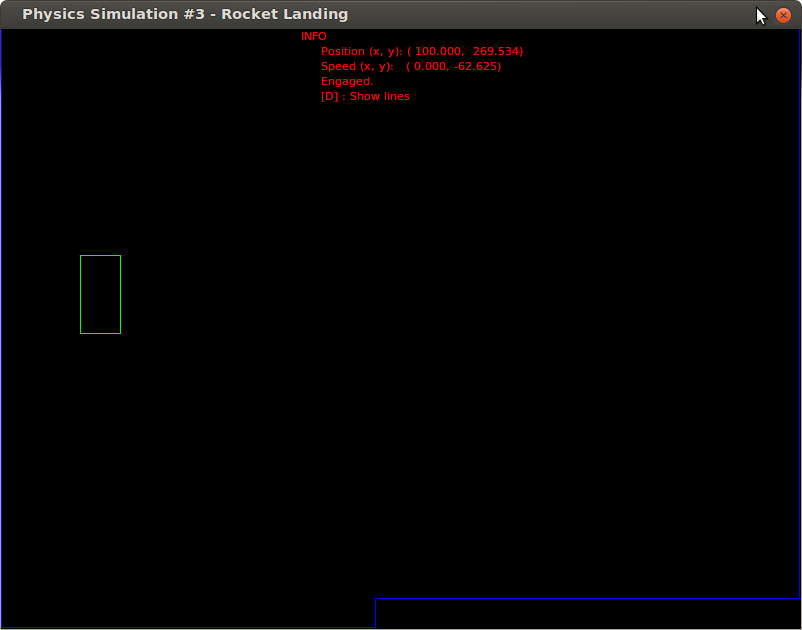
\includegraphics[scale=0.4]{images/lunarLandingE.png}
	\caption{Lunar Landing}
\end{figure}

Baseado no jogo \textit{Lander} TODO, o objetivo é aterrisar um foguete em uma superfície plana com uma velocidade bem pequena. Se o usuário não conseguir diminuir adequadamente a velocidade antes de tocar a superfície, o foguete explode. Em caso de sucesso, ele pousa e uma mensagem de sucesso é exibida. As setas do teclado movimentam o foguete. \\

Com a implementação desta demonstração utilizamos em conjunto o código de detecção de colisão do \textit{Cannonball} com a manipulação de objetos de \textit{Rocket Simulation}. \\

Tanto neste e em outros cenários há a função ''Raio-X'' (tecla 'd'), que mostra ao usuário o esqueleto dos objetos do cenário. Em outras palavras, os \textit{shapes} que estão ativos no \textit{space} da simulação. Mais detalhes na seção \ref{plataforma}.

\begin{figure}[H]
\centering
  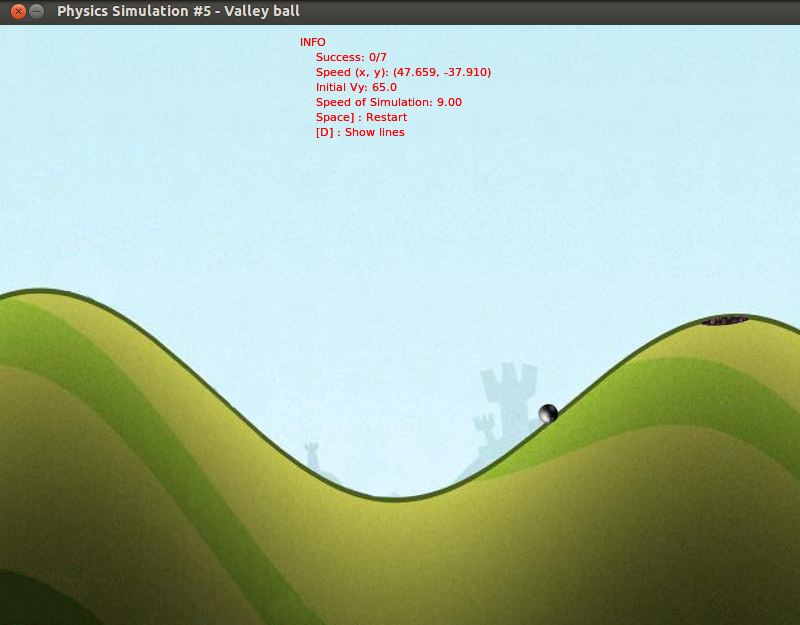
\includegraphics[scale=0.4]{images/valleyball.png}
\end{figure}
\begin{figure}[H]
\centering
  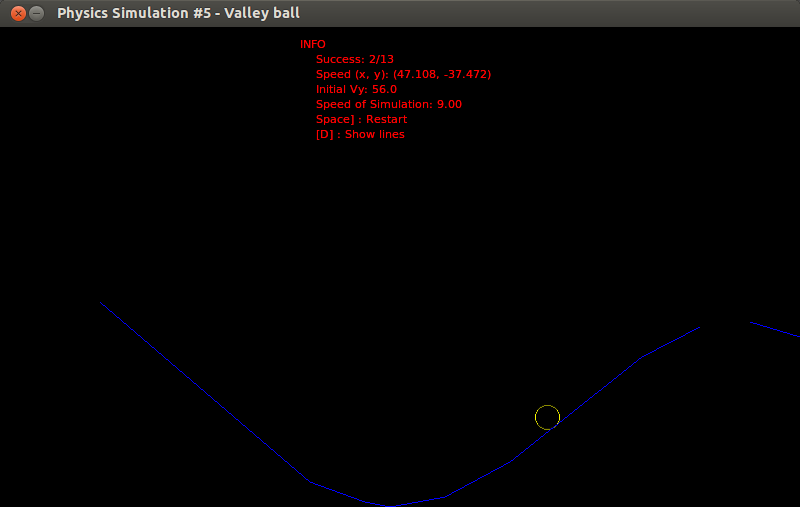
\includegraphics[scale=0.4]{images/valleyballE.png}
  \caption{Valleyball}
\end{figure}

Em \textit{Valleyball}, tentamos ilustrar o Princípio de Conservação da Energia Mecânica e a aplicação da força de atrito. Uma bola é lançada a uma certa altura do chão com velocidade vertical determinada aleatoriamente. Ela então desliza sobre um pequeno vale e dependendo da velocidade inicial ela pode: 1) voltar ao vale e perder velocidade até a situação de repouso; 2) cair em um buraco localizado próximo ao topo de uma montanha; ou 3) prosseguir seu movimento para fora do cenário. O que determina a situação resultante é a velocidade inicial da bola. A tecla de espaço reinicia a simulação com uma nova velocidade para a bola. \\

Nesta demonstração utilizamos pela primeira vez o controle de velocidade da simulação. Dentro de alguns limites, o usuário pode alterar o tamanho do passo da simulação (seção \ref{discretizacao}), tornando a animação mais rápida ou mais lenta. Isso é útil, por exemplo, para acelerar alguma etapa da simulação cujos resultados sejam previsíveis ou pouco interessantes. \\

\begin{figure}[H]
\centering
  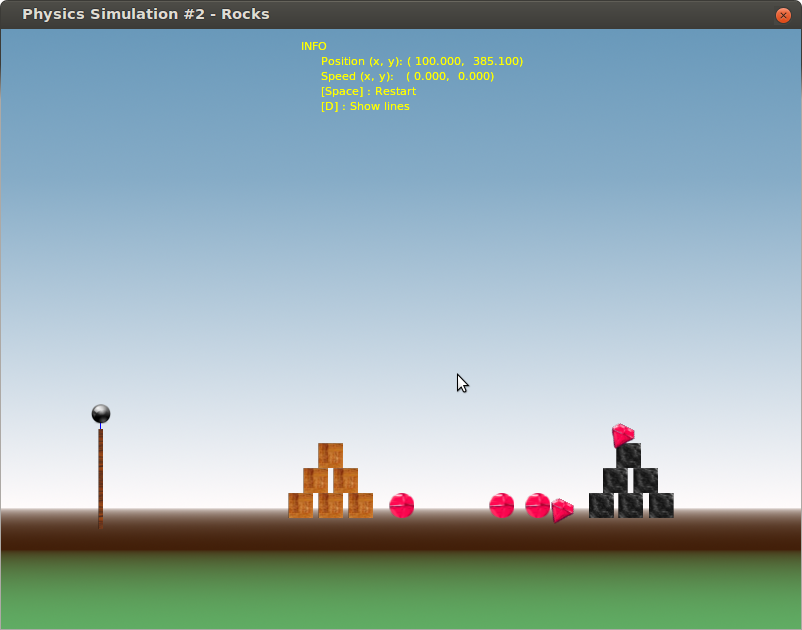
\includegraphics[scale=0.4]{images/rocks.png}
\end{figure}
\begin{figure}[H]
\centering
  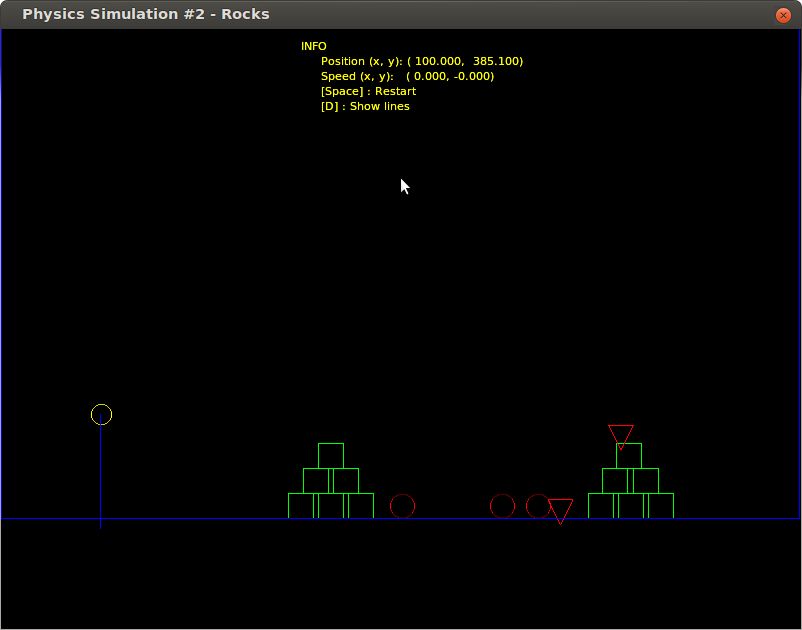
\includegraphics[scale=0.4]{images/rocksE.png}
  \caption{Rocks}
\end{figure}

\textit{Rocks} foi nosso último cenário de demonstração. Parecido com \textit{Cannonball}, o objetivo também é acertar alvos da tela - neste caso os objetos de cor vermelha. Porém é o usuário que determina a força que a bola será atirada, dependendo de quanto ele ''puxar'' a bola segurando e arrastando o \textit{mouse}, de modo semelhante ao comportamento de um estilingue. Com este cenário físico gostaríamos de simular um jogo que recentemente ficou bastante conhecido, o \textit{Angry Birds}. Além dos alvos, há cubos empilhados na tela, sendo estes de dois tipos: de pequena massa (cor de madeira) e de grande massa (cor de pedra). O resultado das colisões entre os objetos da tela variam de acordo com a massa do objeto. \\

Além de ser o único cenário de demonstração que possui interação com o \textit{mouse}, \textit{Rocks} consolidou nosso conhecimento das bibliotecas utilizadas e das modificações que precisávamos fazer para implementar o Physimulation. Em termos de física, a novidade deste cenário é a utilização de Energia Potencial Elástica no lançamento do objeto. 

\subsection{Visualização das animações}
Para visualizar as animações descritas nesta seção, o aluno deve executar o seguinte comando:

\begin{Verbatim}[fontsize=\footnotesize]
	$ cd <<DIR_PHYSIMULATION>>/Simulation
	$ ruby main.rb demos
\end{Verbatim}

\noindent onde {\tt\footnotesize DIR\_PHYSIMULATION} é o diretório em que o Physimulation foi instalado. Em seguida, deve escolher uma das animações listadas no programa e clicar em ''Iniciar''. Caso haja algum problema ao executar qualquer um dos comandos, verificar se os passos da seção \ref{instalacao} (''\nameref{instalacao}'') foram seguidos corretamente.

\begin{figure}[H]
	\centering
	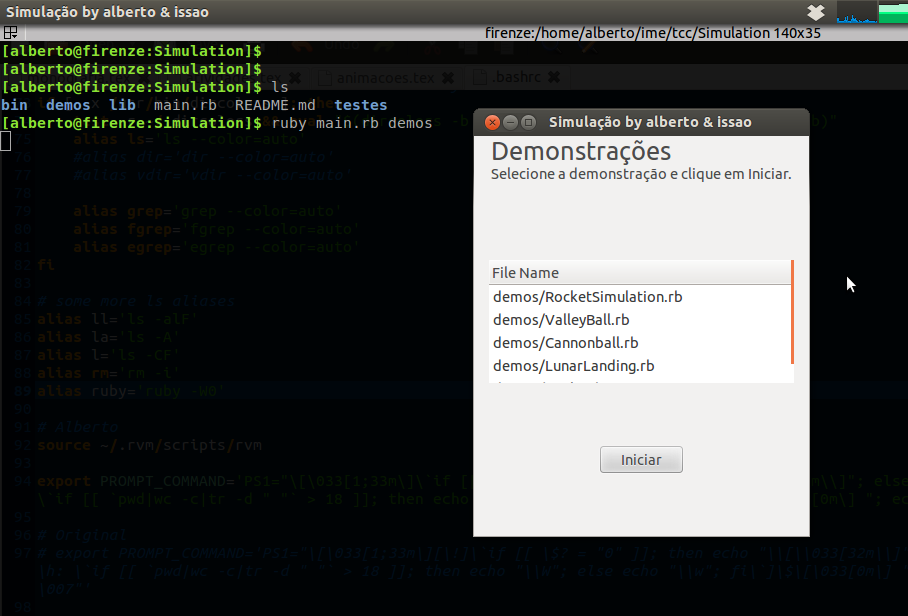
\includegraphics[scale=0.3]{images/demos-menu.png}
	\caption{Menu de demonstrações}
\end{figure}


